\chapter{Method}

\section{Gradient Accumulation with Percentile-Based Sparsification}

In pipeline-parallel training, the neural network is partitioned across multiple devices. During each training step, the upstream device computes a forward pass and sends activations to the downstream device, which computes the loss and sends gradients back. In a standard setup, the full gradient tensor is transmitted after every minibatch. Our method reduces this communication by accumulating gradients locally on the downstream device and selectively transmitting only the most significant values.

\textbf{Accumulation Phase:} The downstream device maintains a gradient accumulator $\mathbf{G} \in \mathbb{R}^{b \times d}$ initialized to zero, where $b$ is the minibatch size and $d$ is the activation dimension. After computing the backward pass for minibatch $i$, the feature gradients are added to the accumulator:
\begin{equation}
\mathbf{G} \leftarrow \mathbf{G} + \nabla_{\mathbf{f}_i} \mathcal{L}
\end{equation}
where $\nabla_{\mathbf{f}_i} \mathcal{L}$ represents gradients with respect to the upstream activations for minibatch $i$.

\textbf{Sparsification and Transmission:} After accumulation, we compute the $p$-th percentile threshold on absolute gradient magnitudes:
\begin{equation}
\tau = \text{quantile}(|\mathbf{G}|, p)
\end{equation}
where $p \in [0, 1]$ is a configurable hyperparameter controlling the compression ratio. We create a binary mask $\mathbf{M}$ and transmit only gradients exceeding the threshold:
\begin{equation}
\mathbf{M}_{ij} = \begin{cases}
1 & \text{if } |\mathbf{G}_{ij}| \geq \tau \\
0 & \text{otherwise}
\end{cases}
\end{equation}

The transmitted representation is sparse: it consists of the indices of selected elements, their gradient values, and the original tensor shape. For a percentile threshold of $p = 0.90$, only 10\% of gradient values are transmitted per minibatch. After transmission, selected gradients are zeroed in the accumulator so they are not retransmitted:
\begin{equation}
\mathbf{G}_{ij} \leftarrow \begin{cases}
0 & \text{if } \mathbf{M}_{ij} = 1 \\
\mathbf{G}_{ij} & \text{otherwise}
\end{cases}
\end{equation}

The upstream device reconstructs the full gradient tensor from the sparse representation and uses it to update its parameters through standard backpropagation.

\textbf{Buffer Decay:} Gradients that remain in the accumulator across many training steps may become stale as the optimization landscape shifts. To mitigate this, we optionally apply an exponential decay factor $\lambda \in (0, 1]$ before adding new gradients:
\begin{equation}
\mathbf{G} \leftarrow \lambda \mathbf{G} + \nabla_{\mathbf{f}_i} \mathcal{L}
\end{equation}
Setting $\lambda = 1.0$ recovers standard accumulation. Values below 1.0 discount older unsent gradients, ensuring the accumulator reflects recent optimization directions rather than outdated signals.

\textbf{Warm Start:} To ensure stable initial training, full gradient communication is maintained for an initial warm start period before enabling sparsification. This allows the network to establish reasonable weights before introducing compression.

The key advantage of this approach for reinforcement learning is that RL algorithms such as PPO reuse collected experience across multiple training epochs, naturally generating repeated gradient signals for similar data. This makes accumulation particularly effective: by deferring transmission until gradients become statistically significant, we reduce communication while preserving the most informative updates.

\section{Experimental Setup}

We train a reinforcement learning agent on the CarRacing-v3 environment, where the goal is to control a car around a racing track. Table~\ref{tab:env-properties} summarizes the environment properties. The observation space consists of $96 \times 96$ RGB images, and the action space is a 3-dimensional continuous vector controlling steering, acceleration, and braking.

\begin{table}[htbp]
\centering
\caption{CarRacing-v3 environment properties.}
\label{tab:env-properties}
\begin{tabular}{ll}
\toprule
\textbf{Property} & \textbf{Value} \\
\midrule
Observation Space & Box(0, 255, (96, 96, 3), uint8) \\
Action Space & Box([-1, 0, 0], 1.0, (3,), float32) \\
\bottomrule
\end{tabular}
\end{table}

We chose this environment because it requires continuous visual perception as input to the policy, mirroring real-world scenarios such as autonomous driving or robotic navigation where high-dimensional image data must be transmitted between distributed components. This makes it a representative testbed for evaluating communication efficiency in pipeline-parallel training, since the CNN feature extractor must process image observations at every timestep and exchange activations and gradients across the network split.

Each observation is stacked as a $4 \times 96 \times 96$ tensor representing four consecutive frames. The agent employs Proximal Policy Optimization (PPO)~\cite{ppo2017} with a total training budget of 800,000 timesteps, where each iteration consists of 4,096 environment steps followed by 10 update epochs with 32 minibatches of size 128.

To simulate pipeline parallelism across bandwidth-constrained devices, we deploy our system using Docker Compose with two containers connected via a bridge network, as shown in Figure~\ref{fig:docker-setup}. Machine~0 hosts the environment and CNN feature extractor, while Machine~1 hosts the actor-critic network. Communication between machines uses PyTorch's distributed RPC framework, which transmits tensors over the network and provides a realistic simulation of inter-device bandwidth limitations.

\begin{figure}[htbp]
\centerline{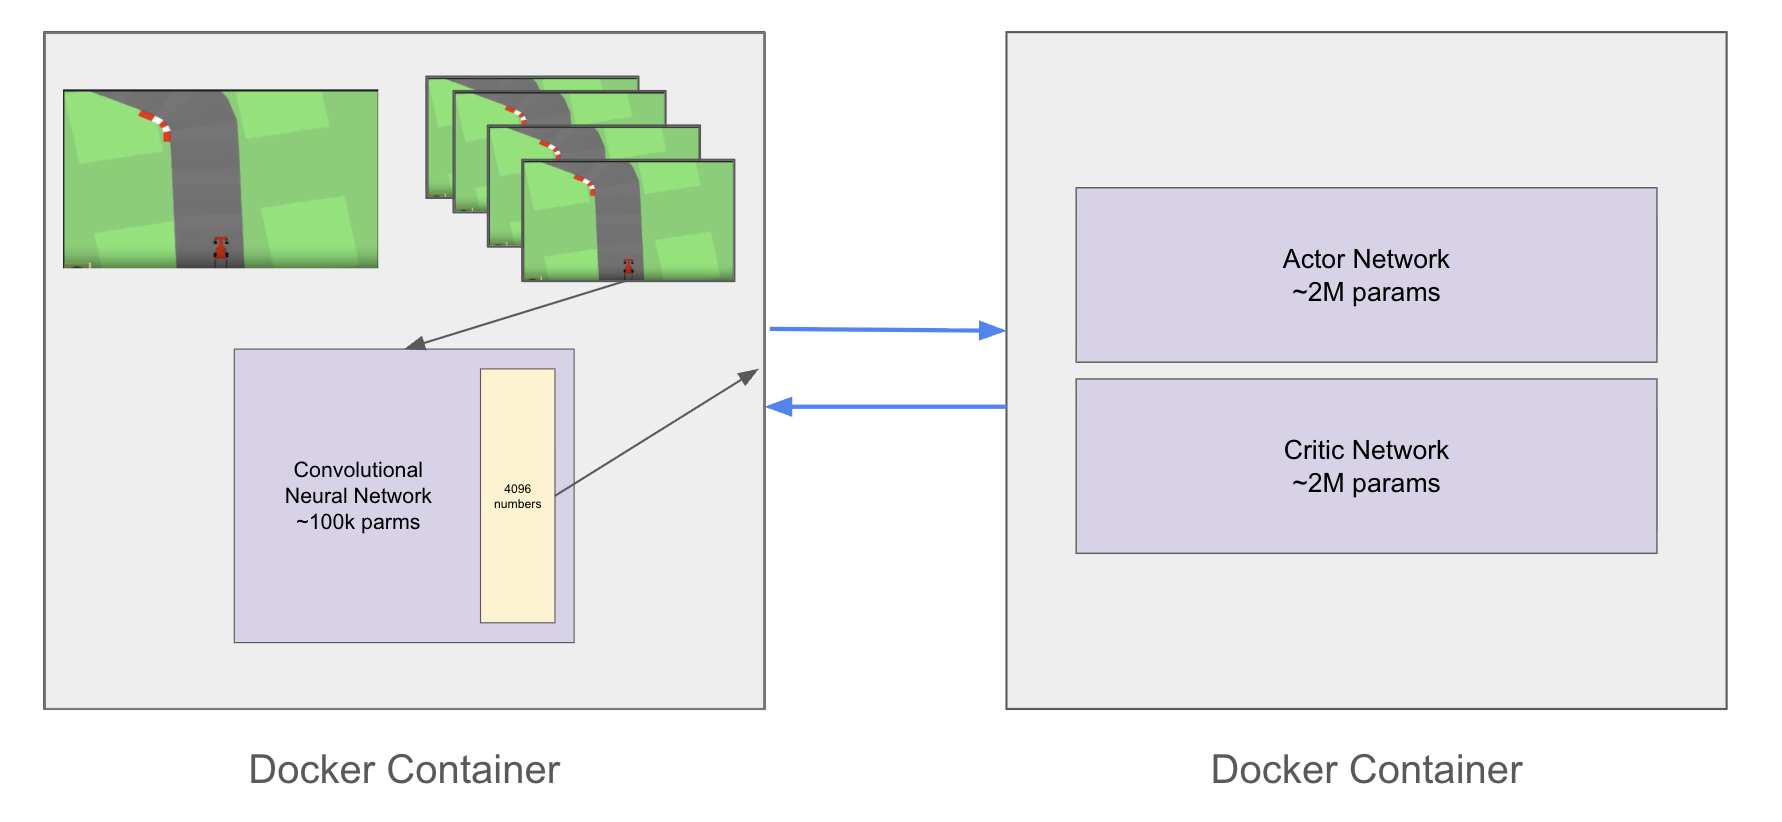
\includegraphics[width=\textwidth]{images/docker_setup.png}}
\caption{Pipeline-parallel deployment using Docker Compose. Machine~0 runs the environment and CNN feature extractor ($\sim$100k parameters), producing a 4096-dimensional feature vector. Machine~1 hosts the actor and critic networks ($\sim$2M parameters each). The two containers exchange activations and gradients over a bridge network.}
\label{fig:docker-setup}
\end{figure}

\section{Network Architecture and Partitioning}

The agent network consists of two components distributed across machines:

\textbf{CNN Feature Extractor (Machine~0):} Processes raw observations through three convolutional layers: Conv2d(4$\rightarrow$32, kernel=8, stride=4), Conv2d(32$\rightarrow$64, kernel=4, stride=2), and Conv2d(64$\rightarrow$64, kernel=3, stride=1), each followed by ReLU activation. The output is flattened to a 4,096-dimensional feature vector. This compression from $4 \times 96 \times 96 = 36,864$ input dimensions to 4,096 features provides a 9$\times$ reduction, significantly lowering communication overhead during policy rollout compared to transmitting raw observations.

\textbf{Actor-Critic Network (Machine~1):} Takes the 4,096-dimensional features as input. The actor head produces a 3-dimensional continuous action (steering, acceleration, brake) through a two-layer MLP (4096$\rightarrow$512$\rightarrow$3) with Gaussian policy parameterization and tanh squashing. The critic head estimates state values through a parallel MLP (4096$\rightarrow$512$\rightarrow$1). Both networks use orthogonal weight initialization for stable training.

During policy rollout, Machine~0 sends 4,096-dimensional feature vectors to Machine~1 for action selection, a 9$\times$ bandwidth savings compared to sending raw $4 \times 96 \times 96$ observations. However, the training phase requires bidirectional communication: forward activations and backward gradients must be exchanged for each minibatch across 10 epochs, creating the 66~GB overhead identified in Chapter~3.

\section{Compression Configuration}

We apply the gradient accumulation method from Section~4.1 to the backward gradient communication from Machine~1 to Machine~0. The accumulator operates on the feature gradient tensor of shape $(128 \times 4096)$, where 128 is the minibatch size and 4,096 is the CNN output dimension. Sparse representations use int16 indices and bfloat16 values to minimize transmission size. The upstream device (Machine~0) reconstructs the sparse gradient tensor and applies it to update CNN parameters through standard backpropagation with gradient clipping (max norm 0.5) and Adam optimization (learning rate $5 \times 10^{-5}$). The warm start period is set to 30,000 timesteps.
